% !TEX root =  master.tex
\section{Entwicklung von Prototypen}
\subsection{Figma}
Zur Erstellung der Prototypen haben wir das Design-Tool \enquote{Figma} verwendet. Dies ist ein Kollaborations-Tool für Designer und funktioniert ähnlich wie Sketch oder Adobe XD, zeichnet sich aber durch zwei signifikante Unterschiede aus\autocite[vgl.][]{?}:
\begin{itemize}[noitemsep]
	\item Es läuft zu 100 \% in Ihrem Browser (keine Installation nötig)
	\item Möglichkeit der Kollaboration mit anderen Personen in Echtzeit
\end{itemize}
Dadurch liefert Figma viele Vorteile, die das gemeinsame Erstellen von Prototypen stark verbessern. Das Tool ist von Designern für Designer entwickelt wurden und einfach im handling. Benutzeroberflächen lassen sich schnell und effektiv designen, ohne viel Zeit in die Einarbeitung des Tools investieren zu müssen. Das kollaboratives Arbeiten in Echtzeit ermöglicht die unkomplizierte Zusammenarbeit am selben Entwurf, ohne extra ein Tool zu installieren oder sich physisch treffen zu müssen. Des weiteren bietet Figma die Möglichkeit, erstellte Screens in vier verschiedenen Formaten zu exportieren als auch Interaktionen hinzuzufügen, um das Projekt im Live-Preview betrachten zu können. Im Live-Preview lassen sich alle zuvor definierten Interaktionen, wie beispielsweise das Navigieren auf einen anderen Screen, ausprobieren und imitieren das Feeling einer echten Anwendung.

\subsection{Mobile First}
Da unsere Zielgruppe eine breite Masse an Menschen beinhaltet, haben wir wert darauf gelegt, dass Xpire möglichst einfach und unkompliziert verwendet werden kann. Einem ansprechenden User Interface sowie einer intuitive User Experience werden daher besondere Bedeutung zugeschrieben.\\
Im Jahr 2015 meldete Google erstmals, dass mehr Suchanfragen über mobile Endgeräte als über Desktop-Geräte erfolgten. Seitdem steigt die der Anteil der Internetnutzer, die auch mit dem Smartphone online gehen, rapide. \footnote{\url{https://de.statista.com/statistik/daten/studie/633698/umfrage/anteil-der-mobilen-internetnutzer-in-deutschland/}} Resultierende aus dieser Entwicklung ist die Wahl des Mobile-First-Ansatzes selbsterklärend. Inzwischen ist nicht mobil-optimierter (responsive) Content ist kaum noch vorstellbar. Mobile Frist lässt sich als neuer Denkansatz im Webdesign definieren. Das Design einer Website wird dabei erstmal in der mobilen Version optimiert, bevor es für größere Bildschirme entwickelt wird. Man arbeitet also von der kleinsten Layout-Version hin zur größten.\autocite[vgl.][]{?}

% Schrittfolge der Screens erklären
\begin{figure}[hbt!]
	\centering
	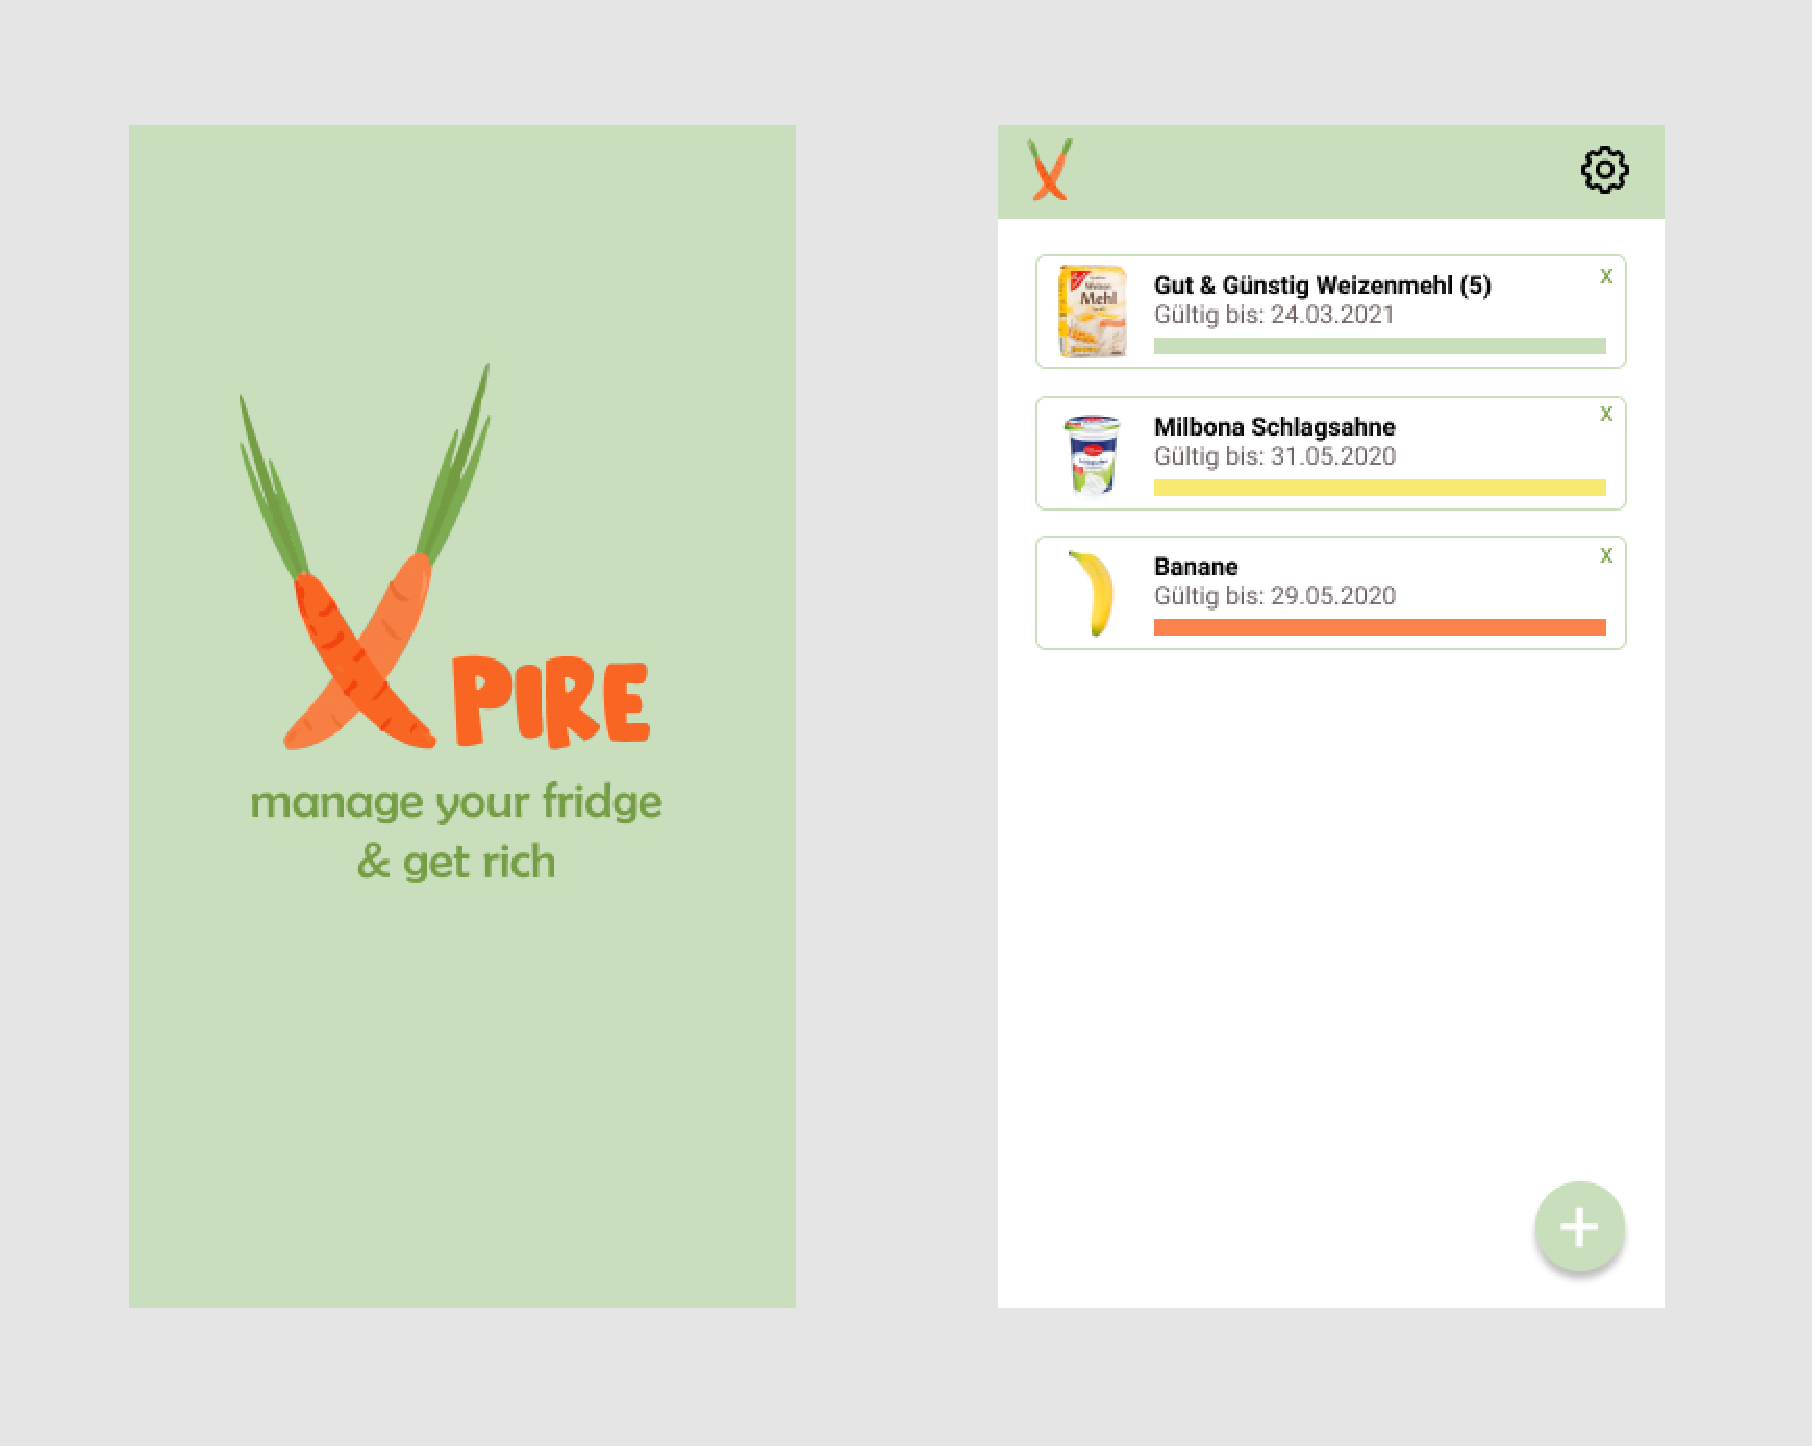
\includegraphics[width=1.0\textwidth]{img/Prototype_01.pdf}
	\caption{Xpire Welcome-Screen und Home-Screen}
	\label{fig:prot1}
\end{figure}
Die Abbildung \ref{fig:prot1} zeigt den \textit{Welcome-Screen} und den \textit{Home-Screen} der Xpire-App. Der \textit{Welcome-Screen} zeigt das Xpire-Logo und wird für einige Sekunden angezeigt, bevor der \textit{Home-Screen} geladen wird. Das Logo mit dem vektorbasierten Grafik- und Zeichenprogramm \enquote{Adobe Illustrator} erstellt. Die gewählte Farbkombination als auch die verwendete Symbolik verleihen dem Logo einen hohen Wiedererkennungswert und ein gewisses Öko-Flair. Das Motto \enquote{Manage your fridge \& get rich} ist nicht nur ein einprägsamer Reim, der sich gut als Werbespruch verwenden lässt, gleichzeitig er eine Anspielung der monetären Ersparnisse dar, die man durch die Benutzung der Xpire-App erzielen kann. 


\begin{figure} 
	\centering
	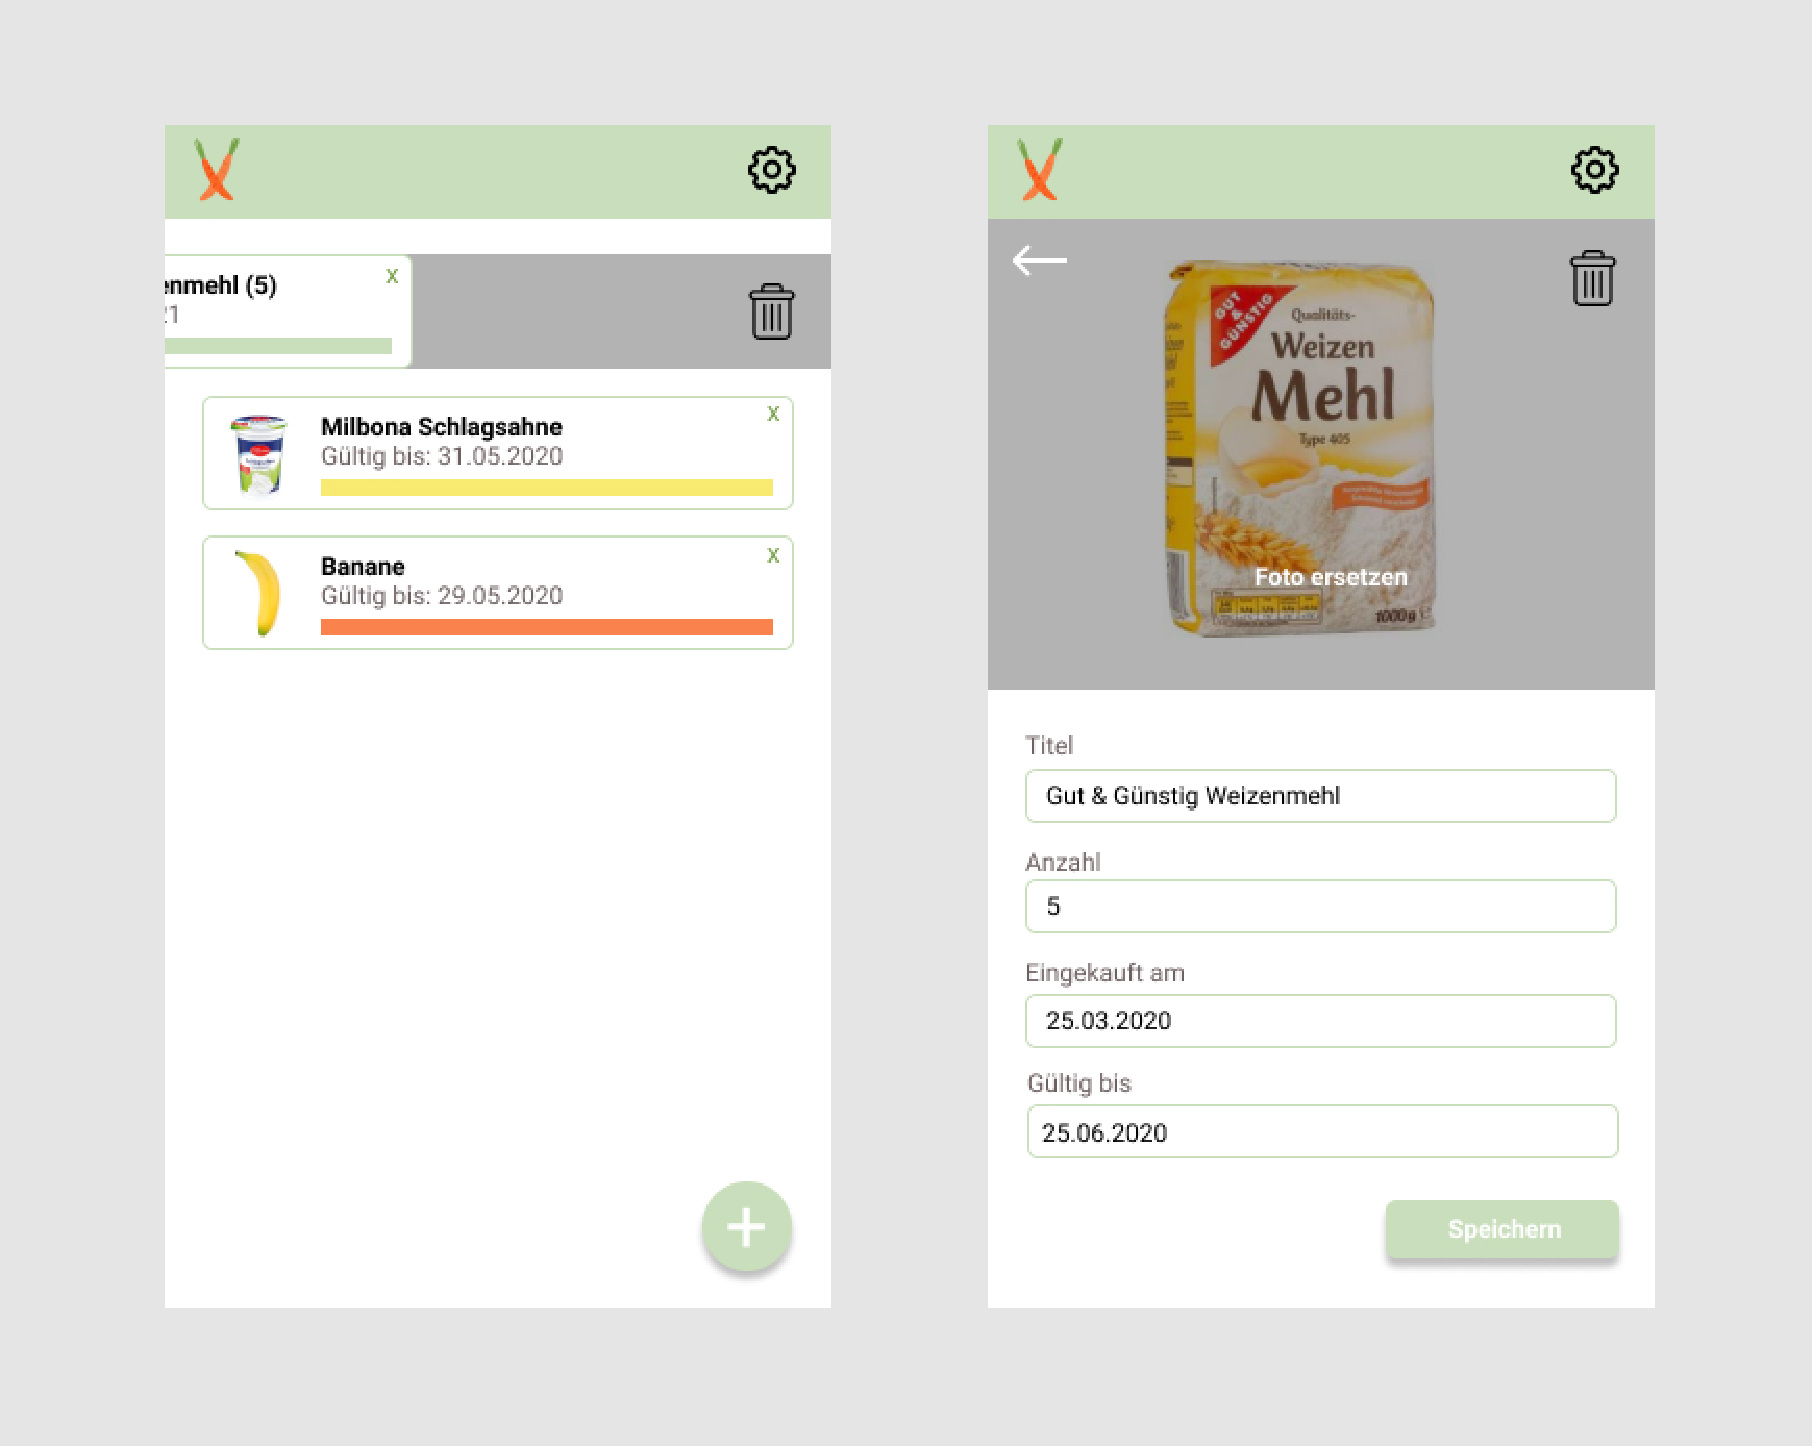
\includegraphics[width=1.0\textwidth]{img/Prototpye_02.pdf}
	\caption{Xpire Delete-Screen und Product-Screen}
	\label{fig:prot2}
\end{figure}
